\chapter{Deque} \label{ch:deque}

By imagining a music player, it has a list of songs which the user can play. To play the songs a user needs to interact with a music player interface. The user can click play, but when they don't like the initial song they can also interact with a next (or previous) button to change songs. When the next song is selected, what should happen when the previous button is clicked? Of course, the previously loaded song should start playing. To implement this functionality a programmer can employ a deque.

Deques allow data insertion and removal from both ends, which can be a little bit confusing to wrap your head around, but that is the functionality needed for such projects.

Going back to \autoref{ch:queue}'s playback chess player, since the game is short, it will be quite fast to push all moves to the queue. Thus it may be more convenient to use a deque for smaller sets of moves. We have a deque with all chess moves inside it, so to play back and forth all that is needed is to have a full deque and an integer variable that stores the number of steps taken and a sign representing the direction from the initial/first move (since players don't usually allow circling to the other end when the current pointer lies on the edge). You can see \autoref{fig:chess-deque} for a better understanding.

\begin{figure}
    \centering
    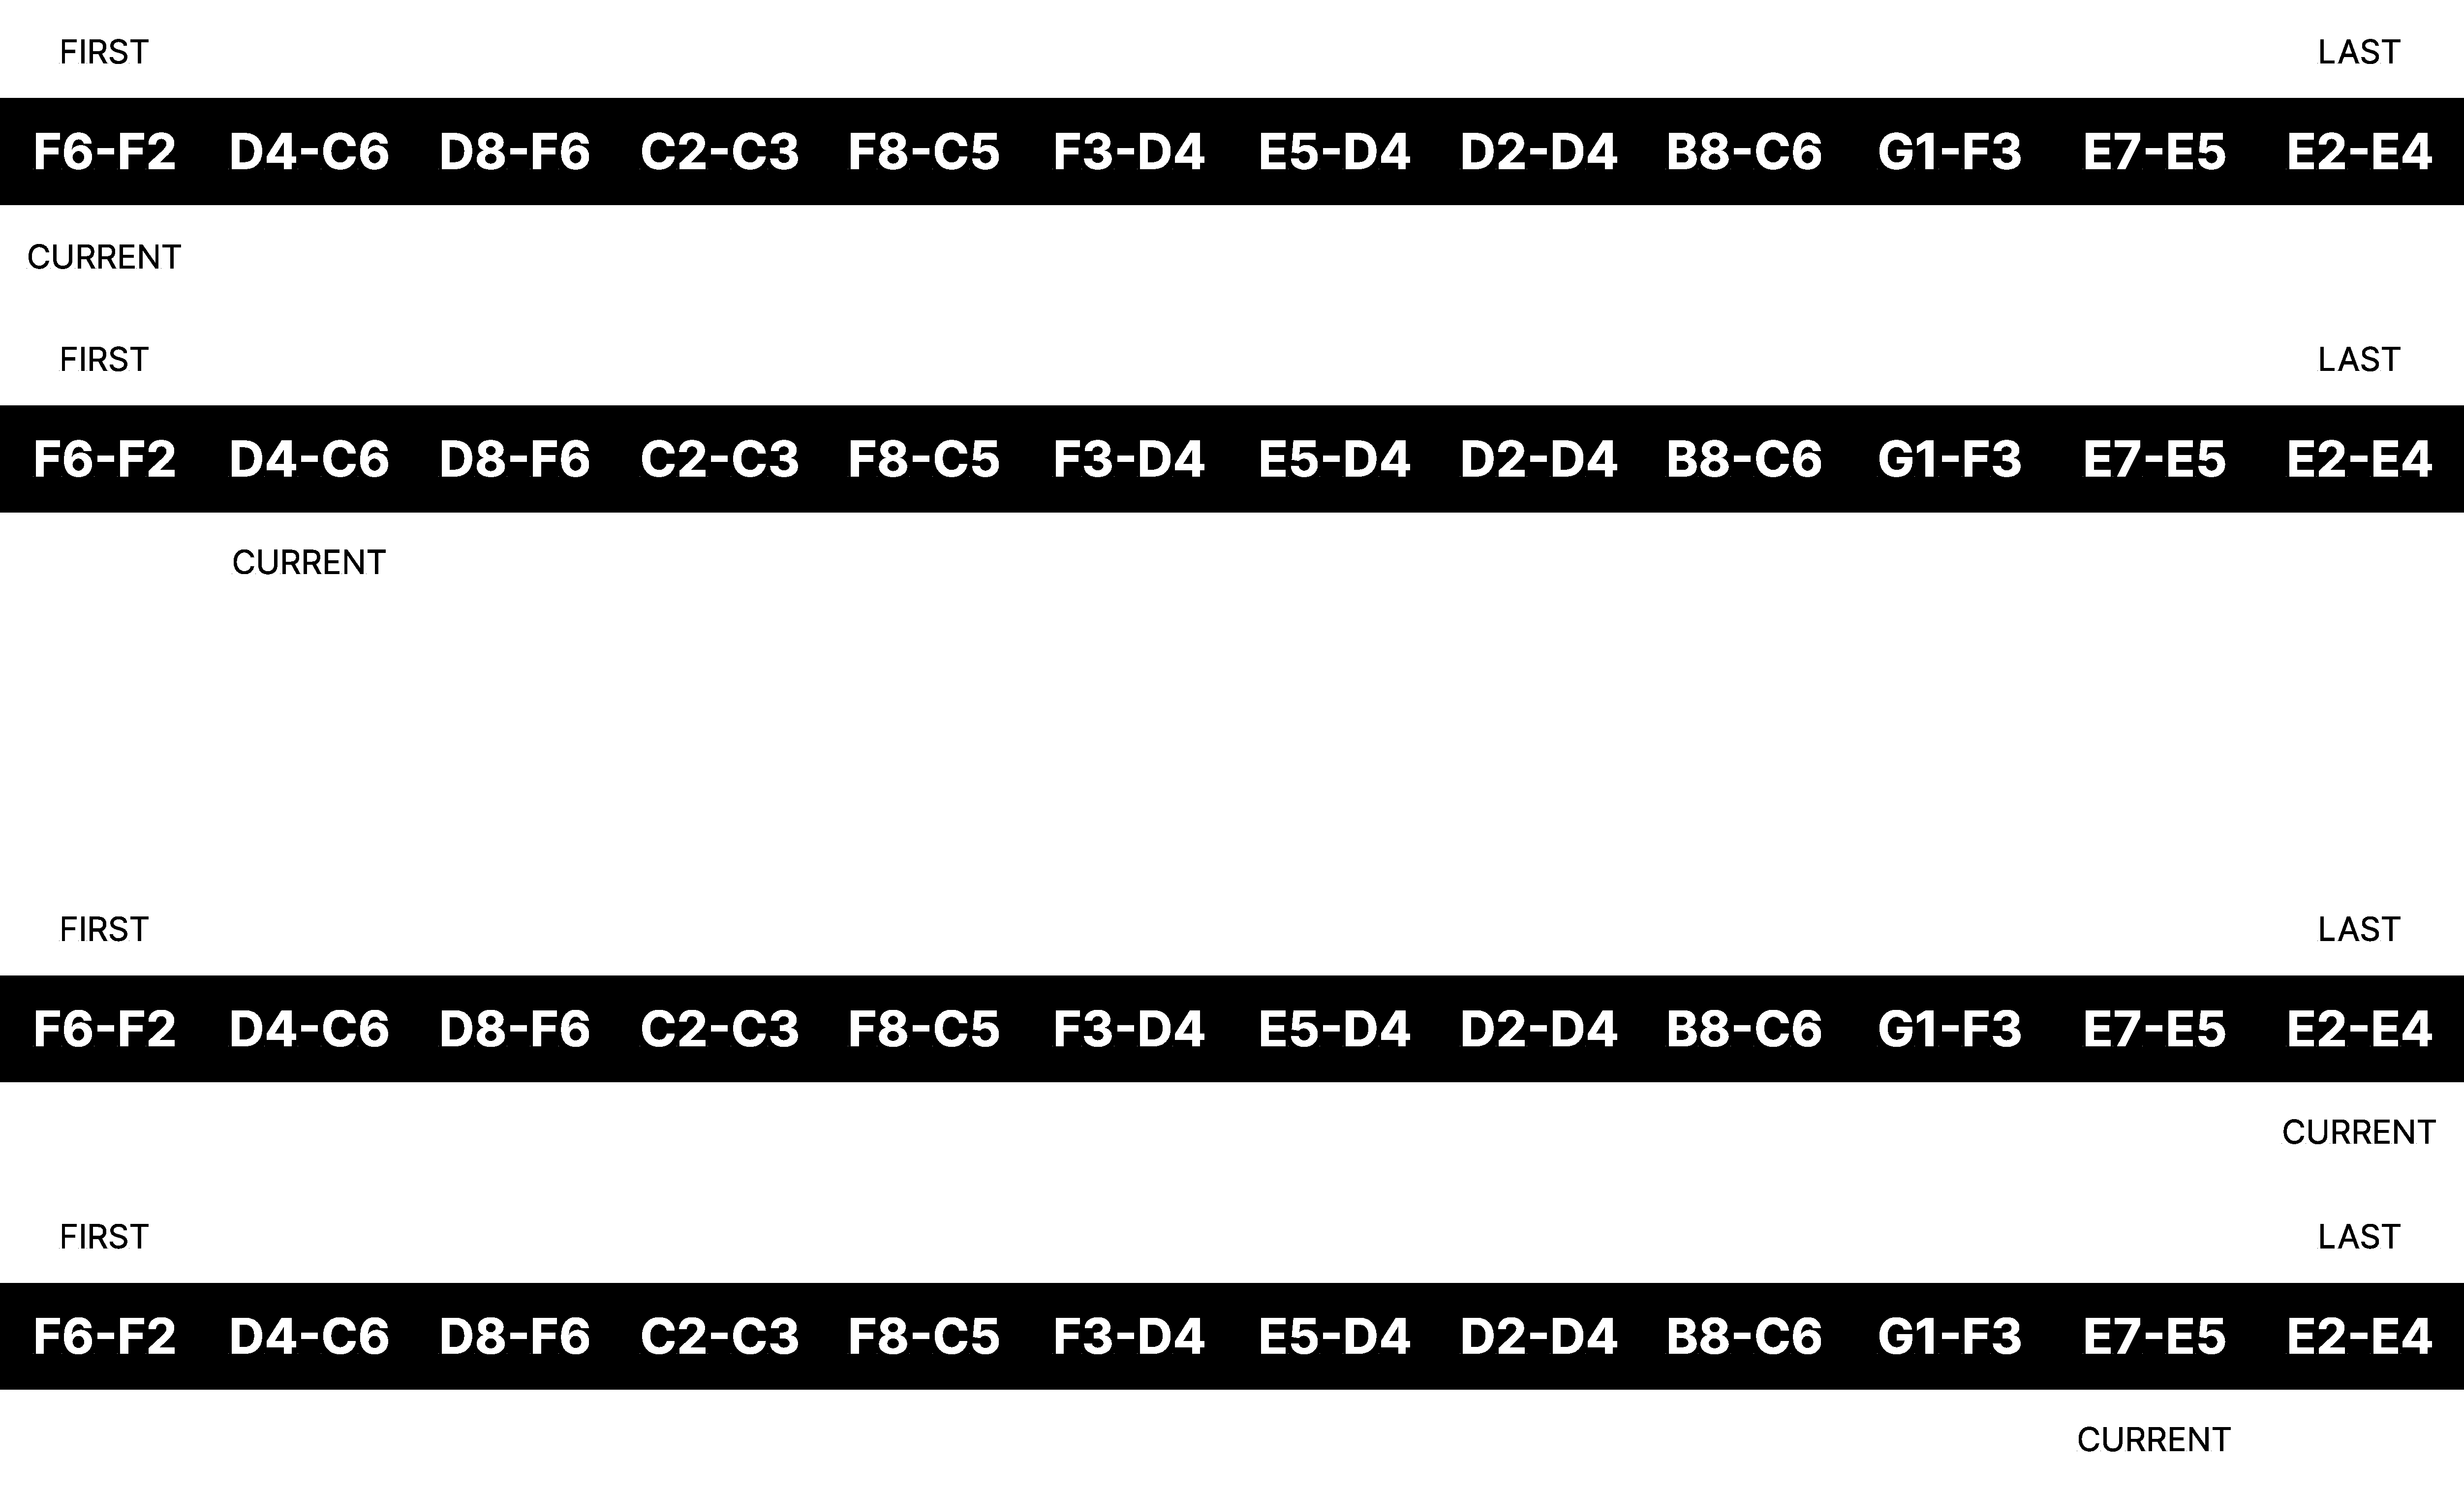
\includegraphics[width=1.0\textwidth]{figures/deque/chess-deque}
    \caption{Visual example of a deque with chess moves and a current index allowing element traversal from first-to-last (top two) and last-to-first (bottom two).}
    \label{fig:chess-deque}
\end{figure}

\section{Implementations of a deque}

The deque also has \sout{three} two implementations. Those implementations are similar to the queue's, but in the case of the array we access elements from two ends. Meanwhile the list implementation relies on doubly linked lists for both two-end access and traversal:

\begin{itemize}
    \item Doubly-linked lists
    \item Static arrays (not dynamic)
\end{itemize}

\subsection{The simple array}

The simplest implementation can include an array of objects and an index pointing to the current objects. To move through them, all that's needed is to increment/decrement the index. But what if the index is zero and decrementing causes the index to become negative, or even worse - underflow? The answer is simple, check if index is zero and then circle back, like this \(current = length - 1\). The simple array-based deque also needs to store the object count - deque length. Overflowing is fixed by checking if the current index is less than deque's length and doing the reverse, by making \(current = 0\). Visual example shown in \autoref{fig:array-deque}.

\begin{figure}
    \centering
    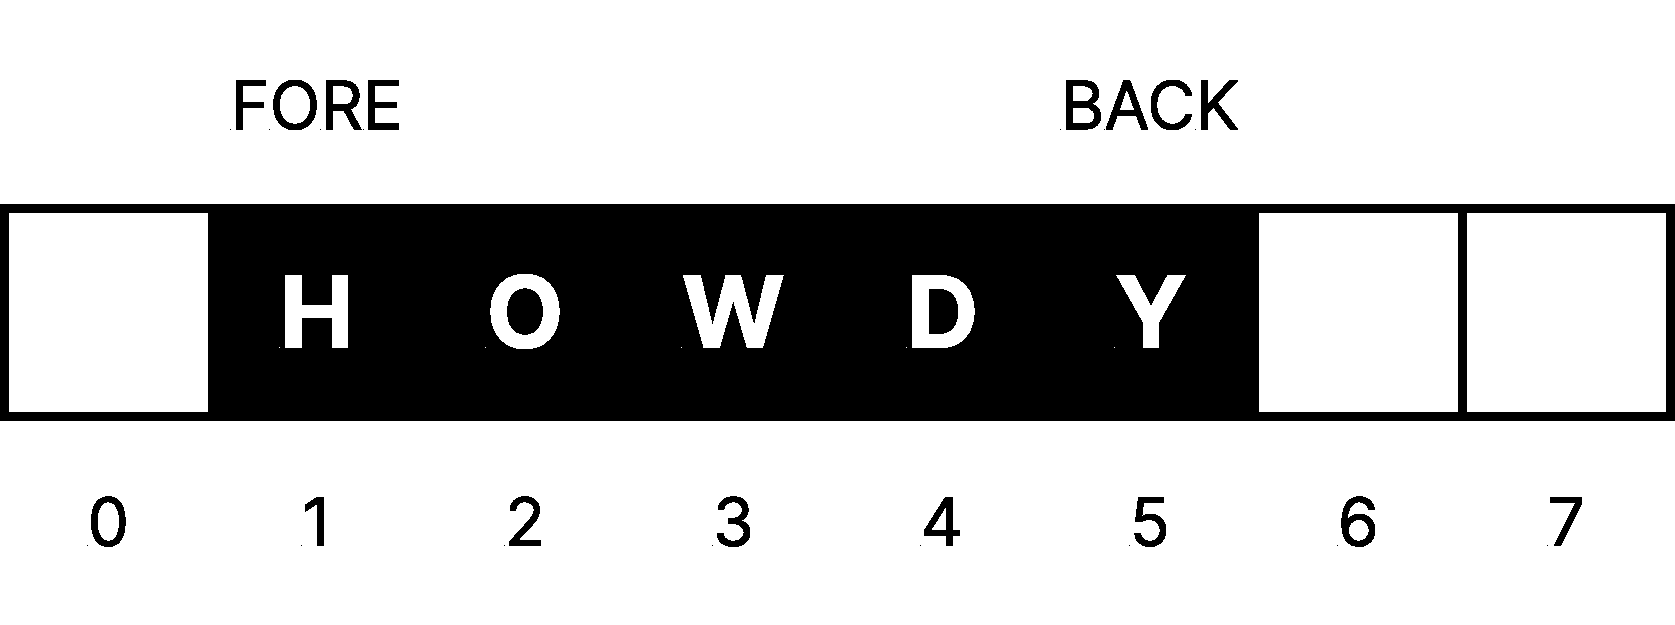
\includegraphics[width=0.6\textwidth]{figures/deque/array-deque}
    \caption{Visual example of an array-based deque with a current front (fore) index allowing element traversal from first-to-last (fore-to-back) and last-to-first (back-to-fore).}
    \label{fig:array-deque}
\end{figure}

\subsection{The complex doubly-linked list}

The most complex implementation can include linked list with one previous and one next pointer. To move through nodes simply get either the head (front) or tail (back) node and iterate through the entire list. To save memory we can make the list circular and only store the head node, since the tail will be accessible through head's previous node pointer, see \autoref{fig:list-deque}.

\begin{figure}
    \centering
    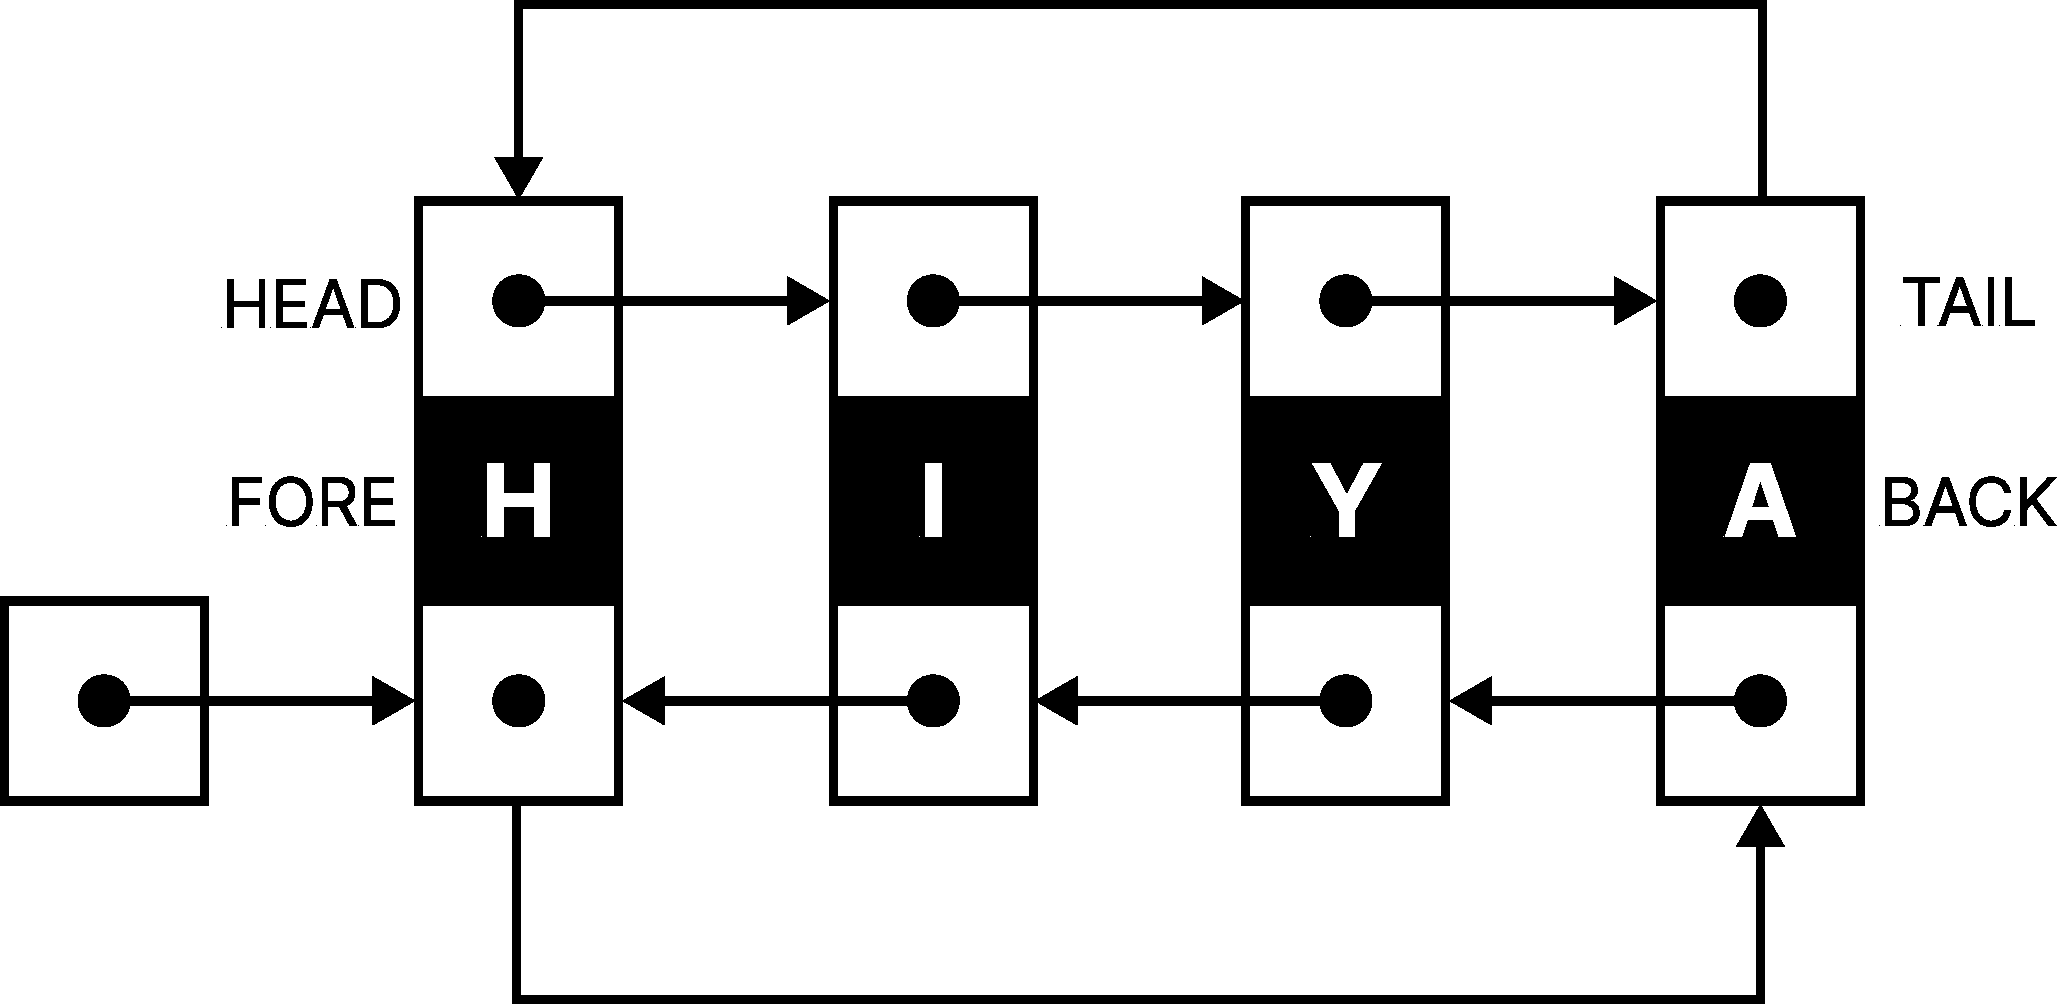
\includegraphics[width=0.7\textwidth]{figures/deque/list-deque}
    \caption{Visual example of a list-based deque with a current front (fore) head node allowing element traversal from first-to-last (fore-to-back) and last-to-first (back-to-fore).}
    \label{fig:list-deque}
\end{figure}

Another memory optimization for doubly-linked lists are XOR linked lists, which store the \texttt{next} and \texttt{previous} pointers as a single XOR pointer of the two, or more accurately, \(combined(A) = next(A) \oplus previous(A)\). To retrieve the next (or previous) node pointer, simply save the head (and tail) pointers as they are and XOR the head's (or tail's) combined pointer, like this \(next(A) = combined(A) \oplus previous(A)\). Again, to save memory we add more operations, but a drawback is that the list is harder to debug. C doesn't allow bitwise operations on pointers, but this can be avoided by casting the pointers to special integer types -- \texttt{intptr\_t} and \texttt{uintptr\_t}.

\begin{infobox}[title=Linux manual page - stdint.h(0p)]
The following type designates a signed integer type with the property that any valid pointer to void can be converted to this type, then converted back to a pointer to void, and the result will compare equal to the original pointer: \texttt{intptr\_t}
\newline
\newline
The following type designates an unsigned integer type with the property that any valid pointer to void can be converted to this type, then converted back to a pointer to void, and the result will compare equal to the original pointer: \texttt{uintptr\_t}
\end{infobox}

\subsection{Doubly-linked list of arrays}

Combining the properties of both lists and arrays I managed create a deque with good locality and growth, look at \autoref{fig:array-list-deque}. Each linked list node is made of a \texttt{previous} \texttt{next} and \text{elements\_array} member. Since it is this good is also gets described in more detail in the next section. Similar to the queue, this deque also relies on finding the perfect middle-ground between allocation speed (finding smaller memory chunks is faster) and locality (the bigger the memory array, the better the locality).

\begin{figure}
    \centering
    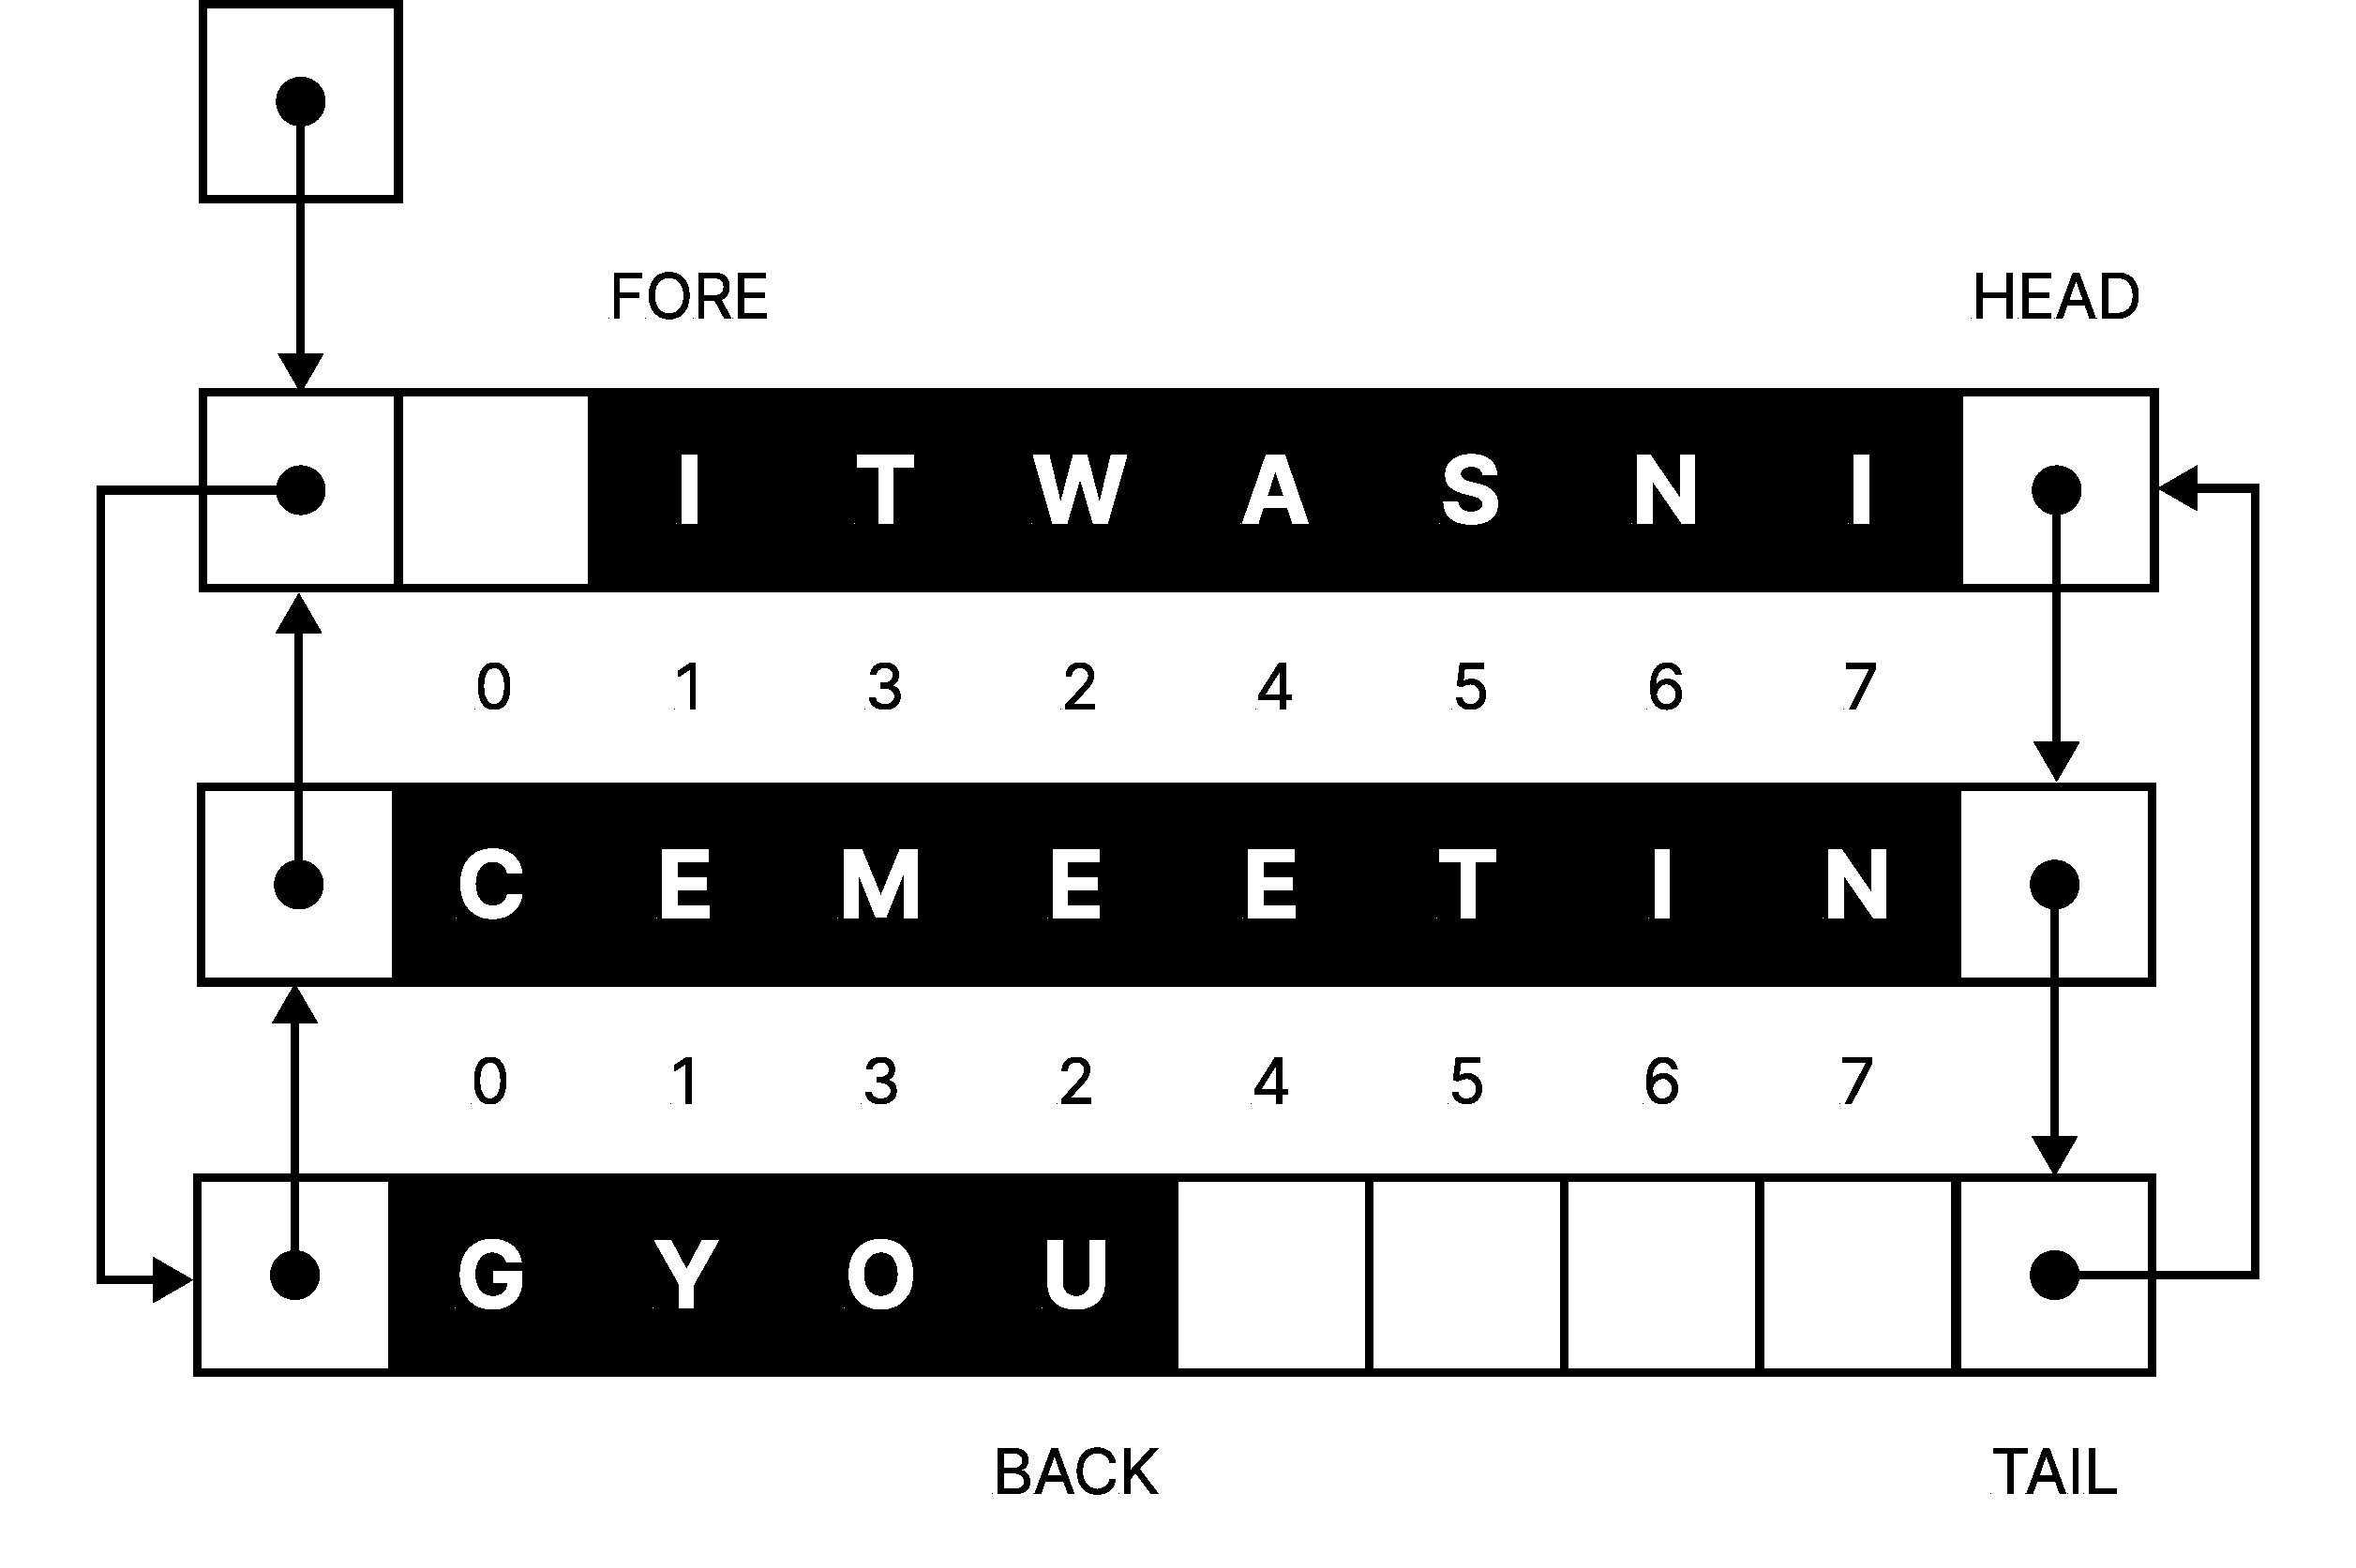
\includegraphics[width=0.7\textwidth]{figures/deque/array-list-deque}
    \caption{Visual example of an array-list based deque with a current front (fore) index allowing element traversal from first-to-last (fore-to-back) and last-to-first (back-to-fore).}
    \label{fig:array-list-deque}
\end{figure}

\section{The infinite deque structure}

The structure consists of a child node structure representing a doubly-linked list node with a flexible array member for storing elements.

The parent structure solely relies on the child head for element storage and traversal. The parent also stores the \texttt{current} front index to simplify front element access in \texttt{peek\_front\_ideque}. Next up is the \texttt{size} member storing individual element size, followed by \texttt{length}. \texttt{length} contains the number of elements in the deque. Lastly, the parent structure stores a pointer to a memory allocator structure for memory management.

\noindent
\begin{minipage}{\linewidth}
\begin{lstlisting}[language=C, style=CodeEditor, label=lst:deque, title=include/sequence/ideque.h]
/// @brief Doubly linked list node for deque structure.
struct infinite_deque_node {
    struct infinite_deque_node * next; // next sibling node
    struct infinite_deque_node * prev; // previous sibling node
    char elements[];                   // elements array with IDEQUE_CHUNK size
};

/// @brief Inifnite deque data structure.
typedef struct infinite_deque {
    struct infinite_deque_node * head;
    size_t current, size, length; // current index, element size and structure length
    memory_s const * allocator;
} ideque_s;
\end{lstlisting}
\end{minipage}

\subsection{Create deque}

Creating a deque means only setting the \texttt{size} member to the size of the element type, and setting the \texttt{allocator} to the \texttt{standard} allocator pointer.

\noindent
\begin{minipage}{\linewidth}
\begin{lstlisting}[language=C, style=CodeEditor, label=lst:create-deque, title=include/sequence/ideque.h]
/// @brief Creates an empty structure.
/// @param size Size of a single element
/// @return Deque structure.
ideque_s create_ideque(size_t const size);
\end{lstlisting}
\end{minipage}

\noindent
\begin{minipage}{\linewidth}
\begin{lstlisting}[language=C, style=CodeEditor, label=lst:create-deque-01, title=source/sequence/ideque.c]
{
    \\ ...
    return (ideque_s) { .size = size, .allocator = allocator, };
}
\end{lstlisting}
\end{minipage}

\subsection{Make deque}

Making the structure is the same as creating it, but with the added option of using a custom memory allocator.

\noindent
\begin{minipage}{\linewidth}
\begin{lstlisting}[language=C, style=CodeEditor, label=lst:make-deque, title=include/sequence/ideque.h]
/// @brief Creates a custom empty structure.
/// @param size Size of a single element.
/// @param allocator Custom allocator structure.
/// @return Deque structure.
ideque_s make_ideque(size_t const size, memory_s const * const allocator);
\end{lstlisting}
\end{minipage}

The memory allocator simply gets set to the \texttt{allocator} member of the structure, while the \texttt{size} member is set the same way as in \texttt{create\_ideque}.

\noindent
\begin{minipage}{\linewidth}
\begin{lstlisting}[language=C, style=CodeEditor, label=lst:make-deque-01, title=source/sequence/ideque.c]
{
    \\ ...
    return (ideque_s) { .size = size, .allocator = allocator, };
}
\end{lstlisting}
\end{minipage}

\subsection{Destroy deque}

Destroying the deque means freeing each element using the \texttt{destroy} function pointer and its \texttt{ad} arguments. The destroy function pointer can either do nothing, set bytes in the element to zero or free the element if it is contains allocated memory.

\noindent
\begin{minipage}{\linewidth}
\begin{lstlisting}[language=C, style=CodeEditor, label=lst:destroy-deque, title=include/sequence/ideque.h]
/// @brief Destroys a structure and its elements, but makes it unusable.
/// @param deque Structure to destroy.
/// @param destroy Function pointer to destroy a single element.
/// @param ad Arguments for destroy function pointer.
void destroy_ideque(ideque_s * const deque, set_fn const destroy, void * const ad);
\end{lstlisting}
\end{minipage}

First a current node pointer is initialized to the head node, then a for loop sets a \texttt{start} index for the current index position for the special case that a node has elements not at the start of the array. All the other nodes have therefore elements starting at index zero, hence the \texttt{start} variable is set to zero after the first iteration.

\noindent
\begin{minipage}{\linewidth}
\begin{lstlisting}[language=C, style=CodeEditor, label=lst:destroy-deque-01, title=source/sequence/ideque.c]
{
    \\ ...
    struct infinite_deque_node * current = deque->head; // save head index as current node
    // for every node in deque list until size is not zero
    for (size_t start = deque->current, remaining = deque->length; remaining; start = 0) {
\end{lstlisting}
\end{minipage}

Following that, the index variable \texttt{i} is set to the \texttt{start} index, and a nested for loop iterates over the elements in the current node, destroying each element using the \texttt{destroy} function pointer. The loop continues until either all remaining elements have been destroyed or the end of the current node's elements array is reached. After destroying the elements, the \texttt{remaining} variable is updated to reflect the number of elements left to destroy.

\noindent
\begin{minipage}{\linewidth}
\begin{lstlisting}[language=C, style=CodeEditor, label=lst:destroy-deque-02, title=source/sequence/ideque.c]
        size_t i = start; // set i outside of nested for loop to save its value
        for (; i < (remaining + start) && i < IDEQUE_CHUNK; ++i) { // destroy each element in node
            destroy(current->elements + (i * deque->size), ad);
        }
        remaining -= (i - start); // subtract absolute value of i and start from deque's size
\end{lstlisting}
\end{minipage}

Lastly, the current node is saved as a temporary variable \texttt{temp} for later freeing. Next the \texttt{current} node pointer is updated to point to the next node in the list. Finally, \texttt{temp} is freed using the defined memory allocator's \texttt{free} function.

\noindent
\begin{minipage}{\linewidth}
\begin{lstlisting}[language=C, style=CodeEditor, label=lst:destroy-deque-03, title=source/sequence/ideque.c]
        struct infinite_deque_node * temp = current; // save current node as temporary to free later
        current = current->next; // go to next node

        deque->allocator->free(temp, deque->allocator->arg); // free temporary current node
    }
\end{lstlisting}
\end{minipage}

All that is left is to zero-out the deque structure, which is done by using \texttt{memset}.

\noindent
\begin{minipage}{\linewidth}
\begin{lstlisting}[language=C, style=CodeEditor, label=lst:destroy-deque-04, title=source/sequence/ideque.c]

    // set everything to zero
    memset(deque, 0, sizeof(ideque_s));
}
\end{lstlisting}
\end{minipage}

\subsection{Clear deque}

Clearing the deque is similar to destroying it, but with the difference being that the structure remains usable. Usability means the deque can still support insertion, deletion and search.

\noindent
\begin{minipage}{\linewidth}
\begin{lstlisting}[language=C, style=CodeEditor, label=lst:clear-deque, title=include/sequence/ideque.h]
/// @brief Clears a structure and destroys its elements, but remains usable.
/// @param deque Structure to destroy.
/// @param destroy Function pointer to destroy a single element.
/// @param ad Arguments for destroy function pointer.
void clear_ideque(ideque_s * const deque, set_fn const destroy, void * const ad);
\end{lstlisting}
\end{minipage}

\noindent
\begin{minipage}{\linewidth}
\begin{lstlisting}[language=C, style=CodeEditor, label=lst:clear-deque-01, title=source/sequence/ideque.c]
{
    struct infinite_deque_node * current = deque->head; // save head index as current node
    // for every node in deque list until size is not zero
    for (size_t start = deque->current, remaining = deque->length; remaining; start = 0) {
        size_t i = start; // set i outside of nested for loop to save its value
        for (; i < (remaining + start) && i < IDEQUE_CHUNK; ++i) { // destroy each element in node
            destroy(current->elements + (i * deque->size), ad);
        }
        remaining -= (i - start); // subtract absolute value of i and start from deque's size

        struct infinite_deque_node * temp = current; // save current node as temporary to free later
        current = current->next; // go to next node

        deque->allocator->free(temp, deque->allocator->arg); // free temporary current node
    }

    deque->current = deque->length = 0;
    deque->head = NULL;
}
\end{lstlisting}
\end{minipage}

\subsection{Copy deque}

Copying is done eon a per-element basis using iteration through each array element and node. The user is able to copy elements in any way they see fit, which also includes deep/shallow copying, and reentrant copies.

\noindent
\begin{minipage}{\linewidth}
\begin{lstlisting}[language=C, style=CodeEditor, label=lst:copy-deque, title=include/sequence/ideque.h]
/// @brief Creates a copy of a structure and all its elements.
/// @param deque Structure to copy.
/// @param copy Function pointer to create a deep/shallow copy of a single element.
/// @param ac Arguments for copy function pointer.
/// @return Deque structure.
ideque_s copy_ideque(ideque_s const * const deque, copy_fn const copy, void * const ac);
\end{lstlisting}
\end{minipage}

We begin by creating a return \texttt{replica} deque structure which gets initialized with the same members as the deque to copy (except the head node pointer of course).

\noindent
\begin{minipage}{\linewidth}
\begin{lstlisting}[language=C, style=CodeEditor, label=lst:copy-deque-01, title=source/sequence/ideque.c]
{
    // ...
    ideque_s replica = {
        .current = deque->current, .size = deque->size, .length = deque->length, .allocator = deque->allocator,
    };
    
\end{lstlisting}
\end{minipage}

First two node pointers are initialized. The first one is a simple current node pointer of the deque head to iterate over. Second is a double pointer to the memory location of the replica for simpler node update.

Next we initialize the for loop with a \texttt{start} index for the special case that the first node can have elements not at the zeroth array position. Continuing on, a remaining length variable is initialized to keep track of how many elements remain to copy.

\noindent
\begin{minipage}{\linewidth}
\begin{lstlisting}[language=C, style=CodeEditor, label=lst:copy-deque-02, title=source/sequence/ideque.c]
    struct infinite_deque_node const * current_deque = deque->head; // save head index as current node
    struct infinite_deque_node ** current_replica = &(replica.head);
    for (size_t start = deque->current, remaining = deque->length; remaining; start = 0) { // while remaining remains
\end{lstlisting}
\end{minipage}

Inside the loop, a new node is allocated and temporary set as \texttt{node} with proper memory size consisting of this formula: 

\[sizeof_{node} + (chunk_{deque} \times size_{element})\]

A copied element counter \texttt{i} is set to \texttt{start} for the inner loop that iterates through each node's array until remaining length or \texttt{IDEQUE\_CHUNK} is reached. Each element is then copied into allocated node's array to the same index. Lastly, the remaining length is decremented by copied size \(i - start\) to fix the \texttt{start} shift.

\noindent
\begin{minipage}{\linewidth}
\begin{lstlisting}[language=C, style=CodeEditor, label=lst:copy-deque-03, title=source/sequence/ideque.c]
        // allocate node for replica
        struct infinite_deque_node * node = deque->allocator->alloc(sizeof(struct infinite_deque_node) + (IDEQUE_CHUNK * deque->size), deque->allocator->arg);
        // ...

        // copy each element from old to replica
        size_t i = start;
        for (; i < IDEQUE_CHUNK && i < remaining + start; ++i) { // operate on each element in node
            copy(node->elements + (i * deque->size), current_deque->elements + (i * deque->size), ac);
        }
        remaining -= (i - start); // decrement remaining size by operated size of current node
\end{lstlisting}
\end{minipage}

Lets see. The worst way to explain this code is to set the reason straight as to why \texttt{current\_replica} is a double pointer. The answer is so that we can directly change the pointer value \texttt{current\_replica} node in the deque struct or member in parent node struct instead of changing the value in the \texttt{current\_replica} variable. First we make \texttt{node} circular to itself from its previous node, together with \texttt{current\_replica}. That all is needed so the code remains general for both the cases of  \texttt{current\_replica} being either the head or body nodes.

Node's next member is set to head's previous pointer, because that guarantees circularity.

Node's previous member is reset to head's previous node, if \texttt{current\_replica} is the head, then circularity is retained, otherwise the node's previous pointer gets corrected.

Head's previous node is set current node as the current node represents the last node added, which is where head's previous must point to. Overall, it is pretty hard code to understand just to avoid a couple \texttt{if} conditions.

\noindent
\begin{minipage}{\linewidth}
\begin{lstlisting}[language=C, style=CodeEditor, label=lst:copy-deque-04, title=source/sequence/ideque.c]
        // current_replica and node's prev will point to node
        (*current_replica) = node->prev = node;
        // node's next points to head (if current_replica is head then node's next points to node)
        node->next = replica.head;
        // node's prev points to head's prev (if current_replica is head then head/prev is node, else prev is previous node)
        node->prev = replica.head->prev;
        // head's prev points to node (if current_copy is head then head/node prev is node, else head prev is last node)
        replica.head->prev = node;
\end{lstlisting}
\end{minipage}

On a simple node, the last thing we do inside the loop is set \texttt{current\_replica} and \texttt{current\_deque} to the next pointer to pointer, and just pointer address, respectively. In the end, the properly initialized \texttt{replica} is returned.

\noindent
\begin{minipage}{\linewidth}
\begin{lstlisting}[language=C, style=CodeEditor, label=lst:copy-deque-05, title=source/sequence/ideque.c]
        current_replica = &((*current_replica)->next); // go to next's node pointer
        current_deque = current_deque->next; // go to next node
    }

    return replica;
}
\end{lstlisting}
\end{minipage}

\subsection{Is empty deque}

Returns true if deque is empty.

\noindent
\begin{minipage}{\linewidth}
\begin{lstlisting}[language=C, style=CodeEditor, label=lst:copy-deque, title=include/sequence/ideque.h]
/// @brief Checks if structure is empty.
/// @param deque Structure to check.
/// @return 'true' if empty, 'false' if not.
bool is_empty_ideque(ideque_s const * const deque);
\end{lstlisting}
\end{minipage}

\noindent
\begin{minipage}{\linewidth}
\begin{lstlisting}[ language=C, style=CodeEditor, label=lst:copy-deque-05, title=source/sequence/ideque.c]
{
    // ...
    return (deque->length == 0);
}
\end{lstlisting}
\end{minipage}

\subsection{Enqueue deque front}

Enqueues element to the front of the deque. The front is defined as the \texttt{head} node's \texttt{current} index element. The inserted element is provided as a pointer \texttt{buffer} parameter.

\noindent
\begin{minipage}{\linewidth}
\begin{lstlisting}[language=C, style=CodeEditor, label=lst:enqueue-front-deque, title=include/sequence/ideque.h]
/// @brief Enqueues a single element to the front of the structure.
/// @param deque Structure to enqueue into.
/// @param buffer Element buffer to enqueue.
void enqueue_front_ideque(ideque_s * const deque, void const * const buffer);
\end{lstlisting}
\end{minipage}

First enqueue front checks if \texttt{current} index is zero. That is because if it is, then a new node needs to be created, pointers need to be redirected and saved to the structure.

\noindent
\begin{minipage}{\linewidth}
\begin{lstlisting}[ language=C, style=CodeEditor, label=lst:enqueue-front-deque-01, title=source/sequence/ideque.c]
{
    // ...
    if (!(deque->current)) { // if deque's previous current 'underflows' in node array due to inserting element to front
\end{lstlisting}
\end{minipage}

The \texttt{current} index is changed to \texttt{IDEQUE\_CHUNK} to later correct it to the last element in node's array during \texttt{current} decrement. Next a new node is allocated using the size of a singular node and chunk size multiplied with the size of a single element.

\noindent
\begin{minipage}{\linewidth}
\begin{lstlisting}[ language=C, style=CodeEditor, label=lst:enqueue-front-deque-02, title=source/sequence/ideque.c]
        deque->current = IDEQUE_CHUNK; // make current into list array chunk size to prevent future underflow

        // allocate node for replica
        struct infinite_deque_node * node = deque->allocator->alloc(sizeof(struct infinite_deque_node) + (IDEQUE_CHUNK * deque->size), deque->allocator->arg);
        // ...
\end{lstlisting}
\end{minipage}

The last thing done inside the \texttt{if} body is to check if a head exists (\texttt{head != NULL}). If head ain't \texttt{NULL}, node is properly redirected so its \texttt{next} pointer becomes head and its \texttt{prev} pointer becomes head's previous. Lastly, head's previous and head previous' next are set to \texttt{node} together with deque's \texttt{head}.

The else condition body makes the node circular and also sets deque's \texttt{head} to \texttt{node}. Which is way simpler to explain and understand than the \texttt{if} body statements.

\noindent
\begin{minipage}{\linewidth}
\begin{lstlisting}[ language=C, style=CodeEditor, label=lst:enqueue-front-deque-03, title=source/sequence/ideque.c]
        if (deque->head) { // if head exists
            node->next = deque->head; // node's next is head
            node->prev = deque->head->prev; // node's previous is tail/head's previous

            deque->head = deque->head->prev = deque->head->prev->next = node;
        } else { // else head does not exist
            deque->head = node->next = node->prev = node; // node's next and previous is node and node becomes head
        }
    }
\end{lstlisting}
\end{minipage}

The last part of the enqueue front function increments the deque's \texttt{length} and decrements \texttt{current} (to make it point to the last element in the array if it was zero (it circles back (to the beginning))). The \texttt{buffer} element is memcopied to deque head element's current position.

\noindent
\begin{minipage}{\linewidth}
\begin{lstlisting}[ language=C, style=CodeEditor, label=lst:enqueue-front-deque-04, title=source/sequence/ideque.c]
    deque->length++; // increment size for new element insertion
    deque->current--; // if current was 0 then current will be 'IDEQUE_CHUNK - 1'
    memcpy(deque->head->elements + (deque->current * deque->size), buffer, deque->size); // copy element into deque's head
}
\end{lstlisting}
\end{minipage}

\subsection{Enqueue deque back}

Enqueues element to the back of the deque. The back position is defined as an element located at the position \(current + length - 1\). The element also gets saved as a \texttt{buffer} to that position.

\noindent
\begin{minipage}{\linewidth}
\begin{lstlisting}[language=C, style=CodeEditor, label=lst:enqueue-back-deque, title=include/sequence/ideque.h]
/// @brief Enqueues a single element to the back of the structure.
/// @param deque Structure to enqueue into.
/// @param buffer Element buffer to enqueue.
void enqueue_back_ideque(ideque_s * const deque, void const * const buffer);
\end{lstlisting}
\end{minipage}

The \texttt{next\_index} represents the next index where the \texttt{buffer} element gets saved relative to the node array. Relativity is achieved with \texttt{IDEQUE\_CHUNK} modulo of \(current + length\).

\noindent
\begin{minipage}{\linewidth}
\begin{lstlisting}[language=C, style=CodeEditor, label=lst:enqueue-back-deque-01, title=source/sequence/ideque.c]
{
    // ...
    size_t const next_index = ((deque->current + deque->length) % IDEQUE_CHUNK);
    if (!next_index) { // if next index to insert into is zero
\end{lstlisting}
\end{minipage}

Under the if condition a new node gets allocated.

\noindent
\begin{minipage}{\linewidth}
\begin{lstlisting}[language=C, style=CodeEditor, label=lst:enqueue-back-deque-02, title=source/sequence/ideque.c]
        struct infinite_deque_node * node = deque->allocator->alloc(sizeof(struct infinite_deque_node) + (IDEQUE_CHUNK * deque->size), deque->allocator->arg);
        // ...
\end{lstlisting}
\end{minipage}

The nested if checks if \texttt{head} is \texttt{NULL}. If true, then the node is inserted just like in \texttt{enqueue\_front\_ideque}, but the node doesn't become the head node (it remains tailly, like... tail-esque). The else body is the same as the enqueue front's, since the head and tail are one and the same.

\noindent
\begin{minipage}{\linewidth}
\begin{lstlisting}[language=C, style=CodeEditor, label=lst:enqueue-back-deque-03, title=source/sequence/ideque.c]
        if (deque->head) { // if head exists
            node->next = deque->head; // node's next is head
            node->prev = deque->head->prev; // node's previous is tail/head's previous

            deque->head->prev = deque->head->prev->next = node; // node is tail's next and head's previous, and node becomes tail
        } else { // else head does not exist
            deque->head = node->next = node->prev = node; // node's next and previous is node and node becomes head
        }
    }
\end{lstlisting}
\end{minipage}

Finally, all that is left is to only increment deque's \texttt{length} and memory copy to head previous', or tail's for short, element array at relative \texttt{next\_index} index index.

\noindent
\begin{minipage}{\linewidth}
\begin{lstlisting}[language=C, style=CodeEditor, label=lst:enqueue-back-deque-04, title=source/sequence/ideque.c]
    deque->length++; // increment size for new element insertion
    memcpy(deque->head->prev->elements + (next_index * deque->size), buffer, deque->size); // copy element into deque's tail
}
\end{lstlisting}
\end{minipage}

\subsection{Dequeue deque front}

The dequeue, unlike the enqueue, removes the front element from the deque, but like the enqueue, the dequeue works with the \texttt{current} index position. The \texttt{buffer} stores the removed element.

\noindent
\begin{minipage}{\linewidth}
\begin{lstlisting}[language=C, style=CodeEditor, label=lst:dequeue-front-deque, title=include/sequence/ideque.h]
/// @brief Dequeues a single element from the front of the structure.
/// @param deque Structure to dequeue from.
/// @param buffer Element buffer to save dequeue.
void dequeue_front_ideque(ideque_s * const deque, void * const buffer);
\end{lstlisting}
\end{minipage}

Now the front-most element gets saved to the buffer and \texttt{current} increments, while the \texttt{length} decrements. Which reflects common deque behavior.

\noindent
\begin{minipage}{\linewidth}
\begin{lstlisting}[language=C, style=CodeEditor, label=lst:dequeue-front-deque-01, title=source/sequence/ideque.c]
{
    // ...
    memcpy(buffer, deque->head->elements + (deque->current * deque->size), deque->size);
    deque->current++; // increment current index since it's removing from front (like a queue)
    deque->length--; // decrement deque's size since front elements gets removed (like a queue)
\end{lstlisting}
\end{minipage}

Next up, if a node becomes empty and needs to be removed, an if condition checks if \texttt{current} was incremented to \texttt{IDEQUE\_CHUNK}, which is an issue. Another way that a node may get removed is if \texttt{length} reaches zero. Back to the issue, if chunk size is reached than \texttt{current} index must be circled back.

\noindent
\begin{minipage}{\linewidth}
\begin{lstlisting}[language=C, style=CodeEditor, label=lst:dequeue-front-deque-02, title=source/sequence/ideque.c]
    // if deque's current index is equal to list chunk or deque is empty free head node
    if ((IDEQUE_CHUNK == deque->current) || !(deque->length)) {
\end{lstlisting}
\end{minipage}

This segment cuts off the \texttt{head} node through pointer list magic. it first saves the \texttt{head} so it doesn't roll off after the cut. Then head next's previous pointer points to tail and tail's next pointer points to head's next.

\noindent
\begin{minipage}{\linewidth}
\begin{lstlisting}[language=C, style=CodeEditor, label=lst:dequeue-front-deque-03, title=source/sequence/ideque.c]
        struct infinite_deque_node * head = deque->head; // temporary save pointer to head node

        head->next->prev = head->prev; // set head next's previous pointer to tail/head's previous
        head->prev->next = head->next; // set tail's next node to head's next node
\end{lstlisting}
\end{minipage}

Deque's \texttt{head} gets either set to its \texttt{next} or \texttt{NULL} if \texttt{length} reaches zero. \texttt{current} is set to zero for recircled, and lastly head node is memory freed.

\noindent
\begin{minipage}{\linewidth}
\begin{lstlisting}[language=C, style=CodeEditor, label=lst:dequeue-front-deque-04, title=source/sequence/ideque.c]
        // if deque's size is zero then set head to NULL, else it's head's next node
        deque->head = deque->length ? deque->head->next : NULL;
        deque->current = 0; // reset current index to zero/beginning

        deque->allocator->free(head, deque->allocator->arg); // free temporary head node
    }
}
\end{lstlisting}
\end{minipage}

\subsection{Dequeue deque back}

Dequeue back dequeues an element from the back of the deque and saves removed element into \texttt{buffer}. The back is defined as a position formula \(current + (length - 1)\) modulo to single chunk size.

\noindent
\begin{minipage}{\linewidth}
\begin{lstlisting}[language=C, style=CodeEditor, label=lst:dequeue-back-deque, title=include/sequence/ideque.h]
/// @brief Dequeues a single element from the back of the structure.
/// @param deque Structure to dequeue from.
/// @param buffer Element buffer to save dequeue.
void dequeue_back_ideque(ideque_s * const deque, void * const buffer);
\end{lstlisting}
\end{minipage}

Initially, the deque length is decreased to represent both removal and for the back position calculation. The position itself is represented by \texttt{back\_index}, which is used to copy the back element into buffer.

\noindent
\begin{minipage}{\linewidth}
\begin{lstlisting}[language=C, style=CodeEditor, label=lst:dequeue-back-deque-01, title=source/sequence/ideque.c]
{
    // ...
    deque->length--; // decrement only size since it's removing from the back
    size_t const back_index = (deque->current + deque->length) % IDEQUE_CHUNK; // calculate back element's index
    memcpy(buffer, deque->head->prev->elements + (back_index * deque->size), deque->size);
\end{lstlisting}
\end{minipage}

If deque is empty, that means only the head/tail node remain as one. Thus the only thing required is the free-up of the node's memory followed by setting the \texttt{current} and \texttt{head} deque struct members to zero/NULL for simpler future enqueues. If length is zero, then \texttt{back\_index} may not be zero and it is a special 'remove node' case.

\noindent
\begin{minipage}{\linewidth}
\begin{lstlisting}[language=C, style=CodeEditor, label=lst:dequeue-back-deque-02, title=source/sequence/ideque.c]
    if (!deque->length) {
        deque->allocator->free(deque->head, deque->allocator->arg); // free head node

        deque->current = 0; // reset current index to 0 if deque is empty
        deque->head = NULL;
\end{lstlisting}
\end{minipage}

The first if is continued by an \texttt{else if} statement, which checks if \texttt{back\_index} is zero, representing the removal of the last element in the node array. This requires freeing up the empty node and return unused memory back to the system. Since this node is the last node in the deque it is saved as a temporary \texttt{tail} for later freeing. Next the tail node is cut off with tail's previous node, and tail's previous node is made to point to deque's head instead of \texttt{tail}. The tail thus becomes lost in the deque, hence it was temporary saved, and all that is left is to free is with the allocator.

\noindent
\begin{minipage}{\linewidth}
\begin{lstlisting}[language=C, style=CodeEditor, label=lst:dequeue-back-deque-03, title=source/sequence/ideque.c]
    } else if (!back_index) { // if current index at back is zero or deque is empty remove empty tail/head
        struct infinite_deque_node * tail = deque->head->prev; // temporary save pointer to head node

        deque->head->prev = tail->prev; // head's tail pointer equals tail's previous
        tail->prev->next = deque->head; // tail previous' next equals head

        deque->allocator->free(tail, deque->allocator->arg); // free temporary tail node
    }
}
\end{lstlisting}
\end{minipage}

\subsection{Peek deque front}

Peeks the front element in the deque at deque's \texttt{current} position.

\noindent
\begin{minipage}{\linewidth}
\begin{lstlisting}[language=C, style=CodeEditor, label=lst:peek-front-deque, title=include/sequence/ideque.h]
/// @brief Peeks a single element from the front of the structure.
/// @param deque Structure to peek.
/// @param buffer Element buffer to save peek.
void peek_front_ideque(ideque_s const * const deque, void * const buffer);
\end{lstlisting}
\end{minipage}

The peeked element is saved into \texttt{buffer} without any removal.

\noindent
\begin{minipage}{\linewidth}
\begin{lstlisting}[language=C, style=CodeEditor, label=lst:peek-front-deque-01, title=source/sequence/ideque.c]
{
    // ...
    memcpy(buffer, deque->head->elements + (deque->current * deque->size), deque->size);
}
\end{lstlisting}
\end{minipage}

\subsection{Peek deque back}

Peeks the back element in the deque at deque's \((current + (length - 1)) \bmod chunk\) position.

\noindent
\begin{minipage}{\linewidth}
\begin{lstlisting}[language=C, style=CodeEditor, label=lst:peek-back-deque, title=include/sequence/ideque.h]
/// @brief Peeks a single element from the back of the structure.
/// @param deque Structure to peek.
/// @param buffer Element buffer to save peek.
void peek_back_ideque(ideque_s const * const deque, void * const buffer);
\end{lstlisting}
\end{minipage}

A \texttt{back\_index} is calculated using the aforementioned formula and element is copied from tail (head's previous) position into \texttt{buffer}. The element is not removed.

\noindent
\begin{minipage}{\linewidth}
\begin{lstlisting}[language=C, style=CodeEditor, label=lst:peek-back-deque-01, title=source/sequence/ideque.c]
{
    // ...
    // calculate back element's location/index and copy it into buffer
    size_t const back_index = (deque->current + deque->length - 1) % IDEQUE_CHUNK;
    memcpy(buffer, deque->head->prev->elements + (back_index * deque->size), deque->size);
}
\end{lstlisting}
\end{minipage}

\subsection{Each deque front}

Each element is iterated in front-to-back order using user-defined \texttt{manage} function pointer and its \texttt{am} arguments.

\noindent
\begin{minipage}{\linewidth}
\begin{lstlisting}[language=C, style=CodeEditor, label=lst:each-front-deque, title=include/sequence/ideque.h]
/// @brief Iterates over each element in structure starting from the front.
/// @param deque Structure to iterate over.
/// @param manage Function pointer to operate on each element reference using element size and arguments.
/// @param am Generic arguments to use in function pointer.
void each_front_ideque(ideque_s const * const deque, manage_fn const manage, void * const am);
\end{lstlisting}
\end{minipage}

A \texttt{current} node variable is set to deque's head in order to be later iterated inside a for loop. Next, a similar approach to destroy/clear deque is used to iterate through each node and its array elements until \texttt{remaining} unvisited elements count reaches zero. Also, a \texttt{start} variable is set to the \texttt{current} deque position for the special head node case where the \texttt{current} position may not lay at zero, while other nodes have the first element at zero.

\noindent
\begin{minipage}{\linewidth}
\begin{lstlisting}[language=C, style=CodeEditor, label=lst:each-front-deque-01, title=source/sequence/ideque.c]
{
    // ...
    struct infinite_deque_node * current = deque->head; // save head node as current pointer
    // while remaining size is not zero
    for (size_t start = deque->current, remaining = deque->length; remaining; start = 0) {
\end{lstlisting}
\end{minipage}

A nested for loop is iterating through each node array element starting at \texttt{start}. Inside the loop the \texttt{manage} function pointer is called with the \texttt{current} node element at \texttt{i} index and \texttt{am} arguments. The reason \texttt{i} is saved outside the for loop is to later subtract it from the \texttt{remaining} unvisited element count. Lastly, the \texttt{current} node is updated with its next sibling to continue the next iteration.

\noindent
\begin{minipage}{\linewidth}
\begin{lstlisting}[language=C, style=CodeEditor, label=lst:each-front-deque-02, title=source/sequence/ideque.c]
        size_t i = start;
        for (; i < (remaining + start) && i < IDEQUE_CHUNK; ++i) { // operate on each element in node
            // if operate returns false then terminate main function
            if (!manage(current->elements + (i * deque->size), am)) {
                return;
            }
        }

        remaining -= (i - start); // decrement remaining size by operated size of current node
        current = current->next; // go to next node
    }
}
\end{lstlisting}
\end{minipage}

\subsection{Each deque back}

Each element is iterated in back-to-front order using user-defined \texttt{manage} function pointer and its \texttt{am} arguments.

\noindent
\begin{minipage}{\linewidth}
\begin{lstlisting}[language=C, style=CodeEditor, label=lst:each-back-deque, title=include/sequence/ideque.h]
/// @brief Iterates over each element in structure starting from the back.
/// @param deque Structure to iterate over.
/// @param manage Function pointer to operate on each element reference using element size and arguments.
/// @param am Generic arguments to use in function pointer.
void each_back_ideque(ideque_s const * const deque, manage_fn const manage, void * const am);
\end{lstlisting}
\end{minipage}

A \texttt{current} node is defined as the deque head, then a \texttt{remaining} size is defined as the deque's length to represent the count of unvisited elements. Next a \texttt{last} index variable is defined to access the last element in the whole structure (not relative to chunk).

\noindent
\begin{minipage}{\linewidth}
\begin{lstlisting}[language=C, style=CodeEditor, label=lst:each-back-deque-01, title=source/sequence/ideque.c]
{
    // ...
    struct infinite_deque_node * current = deque->head; // save head node as current pointer
    for (size_t remaining = deque->length, last = deque->current + deque->length - 1; remaining;) {
\end{lstlisting}
\end{minipage}

Inside the for loop, the current node is updated to its previous node to both start at the tail node and to iterate through the deque in reverse. Later a \texttt{next\_index} is defined to access the node's elements relative to \texttt{IDEQUE\_CHUNK} size. An \texttt{i} index is defined outside another for loop which iterates over each element in node array in reverse. The inner for loop checks if \texttt{i} is less than or equal to \texttt{node\_index} (yes, equal to, because \texttt{node\_index} is a zero-based index \texttt{i} must be equal to, and not a length). The for loop also checks if any \texttt{remaining} elements exist, at the end, the loop increments \texttt{i} and decrements \texttt{remaining}. 

\noindent
\begin{minipage}{\linewidth}
\begin{lstlisting}[language=C, style=CodeEditor, label=lst:each-back-deque-02, title=source/sequence/ideque.c]
        current = current->prev; // fist go to tail and other previous nodes

        size_t const node_index = last % IDEQUE_CHUNK; // calculate last element index in node
        size_t i = 0; // save number of operated elements in node
\end{lstlisting}
\end{minipage}

Inside the inner for loop, the \texttt{manage} function pointer is called for each element in reverse of \texttt{i}, as \(node\_index - i\).

\noindent
\begin{minipage}{\linewidth}
\begin{lstlisting}[language=C, style=CodeEditor, label=lst:each-back-deque-03, title=source/sequence/ideque.c]
        for (; i <= node_index && remaining; ++i, remaining--) { // until node index is reached and elements remain
            // manage on reversed i to start from last element in node
            if (!manage(current->elements + ((node_index - i) * deque->size), am)) {
                return;
            }
        }
        last -= i; // may underflow
    }
}
\end{lstlisting}
\end{minipage}

\subsection{Apply deque}

Turns the deque into an array which the user can manipulate, like sort the elements for example, and the 'changed' array is saved back into the deque. Can also be treated like a continuous buffer for printing or more cache friendly elements access as oppose to the \texttt{each} functions.

\noindent
\begin{minipage}{\linewidth}
\begin{lstlisting}[language=C, style=CodeEditor, label=lst:apply-deque, title=include/sequence/ideque.h]
/// @brief Apply each element in structure into an array to manage.
/// @param deque Structure to map.
/// @param process Function pointer to manage array of elements using structure length, element size and arguments.
/// @param ap Generic arguments to use in function pointer.
void apply_ideque(ideque_s const * const deque, process_fn const process, void * const ap);
\end{lstlisting}
\end{minipage}

Since the deque does not save all element into as a continuous array, the function first allocates an \texttt{elements\_array} of \((length \times size)\) size.

\noindent
\begin{minipage}{\linewidth}
\begin{lstlisting}[language=C, style=CodeEditor, label=lst:apply-deque-01, title=source/sequence/ideque.c]
{
    // ...
    // create elements array to temporary save doubly linked list elements into straight array
    char * elements_array = deque->allocator->alloc(deque->length * deque->size, deque->allocator->arg);
\end{lstlisting}
\end{minipage}

Next the temporary \texttt{elements\_array} is initialized with the elements from the deque using the same front-to-back iteration for loop approach, explained in \texttt{destroy\_ideque}, thus also in \texttt{clear\_ideque}, and \texttt{each\_front\_ideque}. An \texttt{index} variable is used to properly save elements into the \texttt{elements\_array} in zero-based index order.

\noindent
\begin{minipage}{\linewidth}
\begin{lstlisting}[language=C, style=CodeEditor, label=lst:apply-deque-02, title=source/sequence/ideque.c]
    // index increments after getting each element from node
    // remaining count of elements is calculated
    // copying starts from head
    size_t index = 0, remaining = deque->length;
    struct infinite_deque_node * current = deque->head;
    // set start to current and then begin from 0 for all the other elements in array node
    for (size_t start = deque->current; remaining; start = 0) {
        size_t i = start; // temporary save iterator outside for later subtraction

        // copy elements starting from start until either 'relative remaining' or 'array node' size is reached
        for (; i < (remaining + start) && i < IDEQUE_CHUNK; ++i) {
            memcpy(elements_array + (index * deque->size), current->elements + (i * deque->size), deque->size);
            index++;
        }

        remaining -= (i - start); // subtract copied count from remaining size
        current = current->next; // go to next node
    }
\end{lstlisting}
\end{minipage}

After the \texttt{elements\_array} is initialized, the \texttt{process} function pointer is called and the array gets processed by the user function together with \texttt{length} and \texttt{ap} arguments as parameters.

\noindent
\begin{minipage}{\linewidth}
\begin{lstlisting}[language=C, style=CodeEditor, label=lst:apply-deque-03, title=source/sequence/ideque.c]
    process(elements_array, deque->length, ap);
\end{lstlisting}
\end{minipage}

Then the \texttt{index} parameter is reset to zero and the \texttt{elements\_array} elements are saved back into the deque structure using the same deque iteration algorithm.

\noindent
\begin{minipage}{\linewidth}
\begin{lstlisting}[language=C, style=CodeEditor, label=lst:apply-deque-03, title=source/sequence/ideque.c]
    // reset index and remaining and copy back elements from array into each node array
    index = 0, remaining = deque->length, current = deque->head;
    // set start to current and then begin from 0 for all the other elements in array node
    for (size_t start = deque->current; remaining; start = 0) {
        size_t i = start; // temporary save iterator outside for later subtraction

        // copy elements starting from start until either 'relative remaining' or 'array node' size is reached
        for (; i < (remaining + start) && i < IDEQUE_CHUNK; ++i) {
            memcpy(current->elements + (i * deque->size), elements_array + (index * deque->size), deque->size);
            index++;
        }

        remaining -= (i - start); // subtract copied count from remaining size
        current = current->next; // go to next node
    }
\end{lstlisting}
\end{minipage}

Lastly, the {elements\_array} gets deallocated.

\noindent
\begin{minipage}{\linewidth}
\begin{lstlisting}[language=C, style=CodeEditor, label=lst:apply-deque-03, title=source/sequence/ideque.c]
    deque->allocator->free(elements_array, deque->allocator->arg);
}
\end{lstlisting}
\end{minipage}




